%!TEX root = ../documentation.tex


\chapter{Anbindung externer Dienste - Dropbox}

Eines der Ziele von Norbert - Your StudyBuddy ist es Wissensmanagement zu betreiben und somit Wissen zu sammeln und weiterzugeben. Da Informationen und Wissen von Studierenden meistens in Dropbox-Ordner abgelegt werden, wird in diesem Kapitel die technische Anbindung von Dropbox an Norbert beschrieben. Dabei wird zunächst erst allgemein auf den standardisierten Autorisiuerngsprozess \enquote{OAuth} eingegangen und daraufhin die verschiedenen Dropbox Endpoints mit ihren Schnittstellen vorgestellt.


\section{Autorisierungsprozess (OAuth)}

OAuth ist ein offenes Protokoll, dass eine standardisierte und sichere API-Autorisierung für mobile Endgeräte, Webanwendungen und Desktop-Applikationen ermöglicht. Der Benutzer kann über den OAuth-Autorisierungsprozess (Abbildung \ref{04ergebnis:oauth}) einer Anwendung (in diesem Fall Norbert) Zugriff auf gespeicherte Daten erlauben. Dabei loggt sich der Benutzer über die Applikation (Norbert) die Zugriff benötigt, auf dem Dienst, der die freizugebenden Daten speichert, ein (hier Dropbox) und erlaubt der Applikation den Zugriff. Da nicht jede Severinstanz von Norbert über eine Redirect-URL, die nach einem erfolgreichen Login aufgerufen wird, für den OAuth-Prozess verfügt und nicht jeder Severadministrator in der Dropbox Developer Console Norbert - Your StudyBuddy eintragen möchte, wird statt einem Redirect ein Autorisationscode angezeigt, den der Nutzer in Norbert eingeben kann. Norbert kann dann mit diesem Autorisationscode ein wiederverwendbares Access-Token anfragen. Dieses Access-Token dient zur Authentifizierung des Benutzers, sodass kein Benutzername und keine Passwörter ausgetauscht oder gespeichert werden müssen.

\begin{figure}[H]
\centering
	\scalebox{0.5}{\input{uml-diagramms/oauth}}
	\caption{OAuth-Autorisierungsprozess zwischen Norbert und Dropbox.com}
	\label{04ergebnis:oauth}	
\end{figure}


\section{Dropbox Endpoints}

Die Dropbox HTTP-API besteht aus mehreren Endpoints (Abbildung \ref{04ergebnis:dpendpoints}), die jeweils unterschiedliche Funktionen bereitstellen. Alle API-Aufrufe benötigen zu Autorisierung das individuelle Access-Token des Benutzers.

\begin{enumerate}
	\item \textit{dropbox.com:} Über diesen Endpoint/Webseite wird die OAuth-Autorisierung durchgeführt. Es wird nur einmalig zur Generierung des Access-Tokens ein Kontakt zu diesem Endpoint hergestellt.
	
	\item \textit{api.dropboxapi.com (RPC-Endpoint):}  Über die Domain api.dropboxapi.com können RPCs (remote procedure calls) ausgeführt werden. Dabei nimmt dieser Endpoint JSON-Strings im HTTP-Body entgegen und führt je nach aufgerufener URL verschiedene Funktionen aus. Ein RPC-Funktion ist beispielsweise list\_{folder} (\textit{https://api.dropboxapi.com/2/files/list\_{folder}}), die als Parameter einen Pfad erwartet und dann alle im entsprechenden Ordner sich
 befindenden Dateien auflistet. Das Ergebnis der Funktion wird daraufhin wieder im JSON-Format zurückgesendet.
 
 	\item \textit{content.dropboxapi.com (Download/Upload-Endpoint):} Wie der Name schon sagt, können über den Download/Upload-Endpoint Dateien heruntergeladen oder hochgeladen werden. Die benötigten Meta-Daten (Pfad, Datei ID etc.) werden dabei im HTTP-Header als JSON oder URL-Argument übergeben. Funktionsergebnisse werden im JSON-Format im HTTP-Response Header übergeben und Dateien im HTTP-Body übersendet.
\end{enumerate}

\begin{figure}[H]
\centering
	\scalebox{0.5}{% Graphic for TeX using PGF
% Title: C:\Users\Philipp Pütz\Desktop\Vorlesung - Software Engineering I\norbert\dokumentationen\softwareentwurf\uml-diagramms\dropboxendpoints.dia
% Creator: Dia v0.97.2
% CreationDate: Sun Mar 27 17:07:30 2016
% For: Philipp Pütz
% \usepackage{tikz}
% The following commands are not supported in PSTricks at present
% We define them conditionally, so when they are implemented,
% this pgf file will use them.
\ifx\du\undefined
  \newlength{\du}
\fi
\setlength{\du}{15\unitlength}
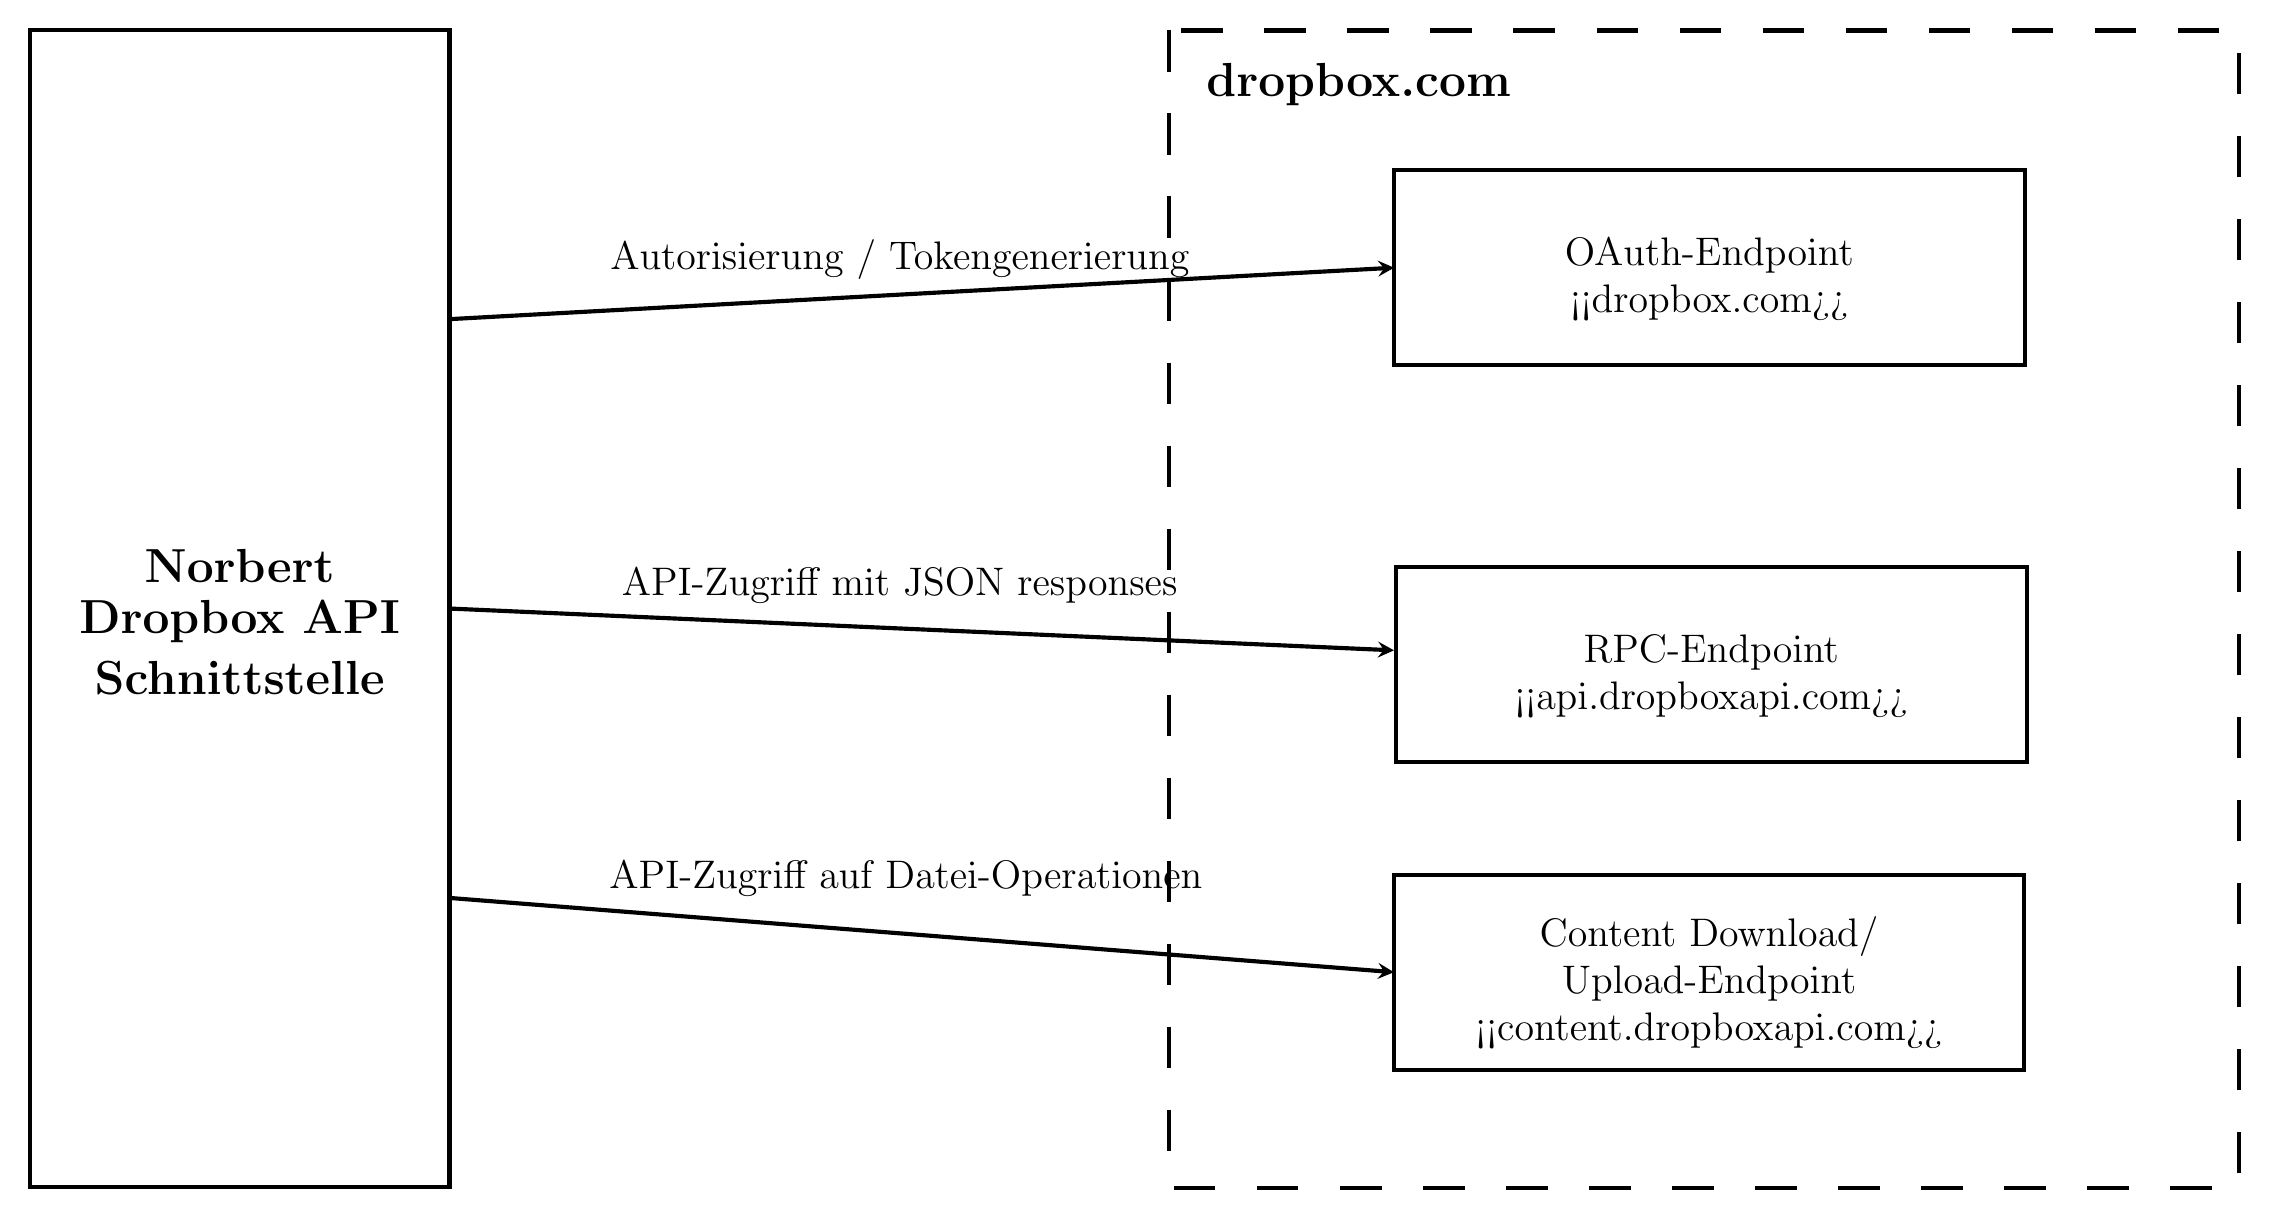
\begin{tikzpicture}
\pgftransformxscale{1.000000}
\pgftransformyscale{-1.000000}
\definecolor{dialinecolor}{rgb}{0.000000, 0.000000, 0.000000}
\pgfsetstrokecolor{dialinecolor}
\definecolor{dialinecolor}{rgb}{1.000000, 1.000000, 1.000000}
\pgfsetfillcolor{dialinecolor}
\definecolor{dialinecolor}{rgb}{1.000000, 1.000000, 1.000000}
\pgfsetfillcolor{dialinecolor}
\fill (8.119868\du,6.074845\du)--(8.119868\du,33.960593\du)--(18.231497\du,33.960593\du)--(18.231497\du,6.074845\du)--cycle;
\pgfsetlinewidth{0.100000\du}
\pgfsetdash{}{0pt}
\pgfsetdash{}{0pt}
\pgfsetmiterjoin
\definecolor{dialinecolor}{rgb}{0.000000, 0.000000, 0.000000}
\pgfsetstrokecolor{dialinecolor}
\draw (8.119868\du,6.074845\du)--(8.119868\du,33.960593\du)--(18.231497\du,33.960593\du)--(18.231497\du,6.074845\du)--cycle;
% setfont left to latex
\definecolor{dialinecolor}{rgb}{0.000000, 0.000000, 0.000000}
\pgfsetstrokecolor{dialinecolor}
\node at (13.175682\du,19.001886\du){\LARGE \textbf{Norbert}};
% setfont left to latex
\definecolor{dialinecolor}{rgb}{0.000000, 0.000000, 0.000000}
\pgfsetstrokecolor{dialinecolor}
\node at (13.175682\du,20.342441\du){\LARGE \textbf{Dropbox API}};
% setfont left to latex
\definecolor{dialinecolor}{rgb}{0.000000, 0.000000, 0.000000}
\pgfsetstrokecolor{dialinecolor}
\node at (13.175682\du,21.682997\du){\LARGE \textbf{Schnittstelle}};
\definecolor{dialinecolor}{rgb}{1.000000, 1.000000, 1.000000}
\pgfsetfillcolor{dialinecolor}
\fill (35.569294\du,6.091693\du)--(35.569294\du,33.977441\du)--(61.330075\du,33.977441\du)--(61.330075\du,6.091693\du)--cycle;
\pgfsetlinewidth{0.100000\du}
\pgfsetdash{{1.000000\du}{1.000000\du}}{0\du}
\pgfsetdash{{1.000000\du}{1.000000\du}}{0\du}
\pgfsetmiterjoin
\definecolor{dialinecolor}{rgb}{0.000000, 0.000000, 0.000000}
\pgfsetstrokecolor{dialinecolor}
\draw (35.569294\du,6.091693\du)--(35.569294\du,33.977441\du)--(61.330075\du,33.977441\du)--(61.330075\du,6.091693\du)--cycle;
% setfont left to latex
\definecolor{dialinecolor}{rgb}{0.000000, 0.000000, 0.000000}
\pgfsetstrokecolor{dialinecolor}
\node at (48.449684\du,20.359289\du){};
% setfont left to latex
\definecolor{dialinecolor}{rgb}{0.000000, 0.000000, 0.000000}
\pgfsetstrokecolor{dialinecolor}
\node[anchor=west] at (48.449684\du,20.034567\du){};
% setfont left to latex
\definecolor{dialinecolor}{rgb}{0.000000, 0.000000, 0.000000}
\pgfsetstrokecolor{dialinecolor}
\node[anchor=west] at (36.193925\du,7.383944\du){\LARGE \textbf{dropbox.com}};
\definecolor{dialinecolor}{rgb}{1.000000, 1.000000, 1.000000}
\pgfsetfillcolor{dialinecolor}
\fill (41.032543\du,19.016385\du)--(41.032543\du,23.709017\du)--(56.222793\du,23.709017\du)--(56.222793\du,19.016385\du)--cycle;
\pgfsetlinewidth{0.100000\du}
\pgfsetdash{}{0pt}
\pgfsetdash{}{0pt}
\pgfsetmiterjoin
\definecolor{dialinecolor}{rgb}{0.000000, 0.000000, 0.000000}
\pgfsetstrokecolor{dialinecolor}
\draw (41.032543\du,19.016385\du)--(41.032543\du,23.709017\du)--(56.222793\du,23.709017\du)--(56.222793\du,19.016385\du)--cycle;
% setfont left to latex
\definecolor{dialinecolor}{rgb}{0.000000, 0.000000, 0.000000}
\pgfsetstrokecolor{dialinecolor}
\node at (48.627668\du,21.071312\du){\Large RPC-Endpoint};
% setfont left to latex
\definecolor{dialinecolor}{rgb}{0.000000, 0.000000, 0.000000}
\pgfsetstrokecolor{dialinecolor}
\node at (48.627668\du,22.200201\du){\Large <<api.dropboxapi.com>>};
% setfont left to latex
\definecolor{dialinecolor}{rgb}{0.000000, 0.000000, 0.000000}
\pgfsetstrokecolor{dialinecolor}
\node[anchor=west] at (49.690330\du,18.401183\du){};
\definecolor{dialinecolor}{rgb}{1.000000, 1.000000, 1.000000}
\pgfsetfillcolor{dialinecolor}
\fill (40.983369\du,26.431875\du)--(40.983369\du,31.124507\du)--(56.165869\du,31.124507\du)--(56.165869\du,26.431875\du)--cycle;
\pgfsetlinewidth{0.100000\du}
\pgfsetdash{}{0pt}
\pgfsetdash{}{0pt}
\pgfsetmiterjoin
\definecolor{dialinecolor}{rgb}{0.000000, 0.000000, 0.000000}
\pgfsetstrokecolor{dialinecolor}
\draw (40.983369\du,26.431875\du)--(40.983369\du,31.124507\du)--(56.165869\du,31.124507\du)--(56.165869\du,26.431875\du)--cycle;
% setfont left to latex
\definecolor{dialinecolor}{rgb}{0.000000, 0.000000, 0.000000}
\pgfsetstrokecolor{dialinecolor}
\node at (48.574619\du,27.922357\du){\Large Content Download/};
% setfont left to latex
\definecolor{dialinecolor}{rgb}{0.000000, 0.000000, 0.000000}
\pgfsetstrokecolor{dialinecolor}
\node at (48.574619\du,29.051246\du){\Large Upload-Endpoint};
% setfont left to latex
\definecolor{dialinecolor}{rgb}{0.000000, 0.000000, 0.000000}
\pgfsetstrokecolor{dialinecolor}
\node at (48.574619\du,30.180135\du){\Large <<content.dropboxapi.com>>};
\definecolor{dialinecolor}{rgb}{1.000000, 1.000000, 1.000000}
\pgfsetfillcolor{dialinecolor}
\fill (40.986152\du,9.460898\du)--(40.986152\du,14.153530\du)--(56.176402\du,14.153530\du)--(56.176402\du,9.460898\du)--cycle;
\pgfsetlinewidth{0.100000\du}
\pgfsetdash{}{0pt}
\pgfsetdash{}{0pt}
\pgfsetmiterjoin
\definecolor{dialinecolor}{rgb}{0.000000, 0.000000, 0.000000}
\pgfsetstrokecolor{dialinecolor}
\draw (40.986152\du,9.460898\du)--(40.986152\du,14.153530\du)--(56.176402\du,14.153530\du)--(56.176402\du,9.460898\du)--cycle;
% setfont left to latex
\definecolor{dialinecolor}{rgb}{0.000000, 0.000000, 0.000000}
\pgfsetstrokecolor{dialinecolor}
\node at (48.581277\du,11.515825\du){\Large OAuth-Endpoint};
% setfont left to latex
\definecolor{dialinecolor}{rgb}{0.000000, 0.000000, 0.000000}
\pgfsetstrokecolor{dialinecolor}
\node at (48.581277\du,12.644714\du){\Large <<dropbox.com>>};
\pgfsetlinewidth{0.100000\du}
\pgfsetdash{}{0pt}
\pgfsetdash{}{0pt}
\pgfsetbuttcap
{
\definecolor{dialinecolor}{rgb}{0.000000, 0.000000, 0.000000}
\pgfsetfillcolor{dialinecolor}
% was here!!!
\pgfsetarrowsend{stealth}
\definecolor{dialinecolor}{rgb}{0.000000, 0.000000, 0.000000}
\pgfsetstrokecolor{dialinecolor}
\draw (18.231497\du,13.046282\du)--(40.986152\du,11.807214\du);
}
% setfont left to latex
\definecolor{dialinecolor}{rgb}{0.000000, 0.000000, 0.000000}
\pgfsetstrokecolor{dialinecolor}
\node[anchor=west] at (21.832636\du,11.607819\du){\Large Autorisierung / Tokengenerierung};
\pgfsetlinewidth{0.100000\du}
\pgfsetdash{}{0pt}
\pgfsetdash{}{0pt}
\pgfsetbuttcap
{
\definecolor{dialinecolor}{rgb}{0.000000, 0.000000, 0.000000}
\pgfsetfillcolor{dialinecolor}
% was here!!!
\pgfsetarrowsend{stealth}
\definecolor{dialinecolor}{rgb}{0.000000, 0.000000, 0.000000}
\pgfsetstrokecolor{dialinecolor}
\draw (18.231497\du,20.017719\du)--(40.983172\du,21.024444\du);
}
% setfont left to latex
\definecolor{dialinecolor}{rgb}{0.000000, 0.000000, 0.000000}
\pgfsetstrokecolor{dialinecolor}
\node[anchor=west] at (22.111685\du,19.457832\du){\Large API-Zugriff mit JSON responses};
\pgfsetlinewidth{0.100000\du}
\pgfsetdash{}{0pt}
\pgfsetdash{}{0pt}
\pgfsetbuttcap
{
\definecolor{dialinecolor}{rgb}{0.000000, 0.000000, 0.000000}
\pgfsetfillcolor{dialinecolor}
% was here!!!
\pgfsetarrowsend{stealth}
\definecolor{dialinecolor}{rgb}{0.000000, 0.000000, 0.000000}
\pgfsetstrokecolor{dialinecolor}
\draw (18.231497\du,26.989156\du)--(40.983369\du,28.778191\du);
}
% setfont left to latex
\definecolor{dialinecolor}{rgb}{0.000000, 0.000000, 0.000000}
\pgfsetstrokecolor{dialinecolor}
\node[anchor=west] at (26.329874\du,19.411982\du){};
% setfont left to latex
\definecolor{dialinecolor}{rgb}{0.000000, 0.000000, 0.000000}
\pgfsetstrokecolor{dialinecolor}
\node[anchor=west] at (21.813661\du,26.521745\du){\Large API-Zugriff auf Datei-Operationen};
\end{tikzpicture}
}
	\caption{API-Zugriffe über die Dropbox-Endpoints}
	\label{04ergebnis:dpendpoints}	
\end{figure}

%\section{Webhooks \& Benachrichtigungen}
%
%Die Benutzer von Norbert wollen nicht jedes mal wenn Sie Änderungen an ihrer Dropbox vornehmen, diese manuell an Norbert weitermelden. Stattdessen sollte dies automatisch vonstatten gehen. Dazu existieren zwei Architekturansätze:
%
%\begin{enumerate}
%	\item Norbert \enquote{scannt} automatisch in bestimmten Zeitintervallen die Dropbox nach Änderungen (keine zusätzlichen Komponenten nötig).
%	
%	\item Dropbox benachrichtigt Norbert vollautomatisch bei Änderungen mittels Webhooks.
%\end{enumerate}
%
%Beide Ansätze erfüllen ihren Zweck und haben ihre Vor- und Nachteile. Der erste Ansatz ist einfach umzusetzen und kann beispielsweise jede Nacht ausgeführt werden. Doch der zweite Ansatz kann Norbert schneller auf Änderungen reagieren lassen, benötigt aber zusätzliche Komponenten. Da schnelles Wissensmanagement im Vordergrund steht wird in diesem Kapitel auf die benötigten Komponenten zur Implementierung des zweiten Ansatzes eingegangen.
%
%Webhooks sind ein nicht standardisiertes Verfahren um Echtzeitbenachrichtigungen zwischen Servern und Software auszutauschen. Die Kommunikation findet dabei über HTTP-POST-Requests statt. Abbildung \ref{04ergebnis:webhook} zeigt den Ablauf der Benachrichtigungen und die daraufhin angestoßenen Prozesse.
%
%\begin{figure}[H]
%\centering
%	\scalebox{0.5}{% Graphic for TeX using PGF
% Title: C:\Users\Philipp Pütz\Desktop\Vorlesung - Software Engineering I\norbert\dokumentationen\softwareentwurf\uml-diagramms\webhook.dia
% Creator: Dia v0.97.2
% CreationDate: Mon Mar 28 11:55:40 2016
% For: Philipp Pütz
% \usepackage{tikz}
% The following commands are not supported in PSTricks at present
% We define them conditionally, so when they are implemented,
% this pgf file will use them.
\ifx\du\undefined
  \newlength{\du}
\fi
\setlength{\du}{15\unitlength}
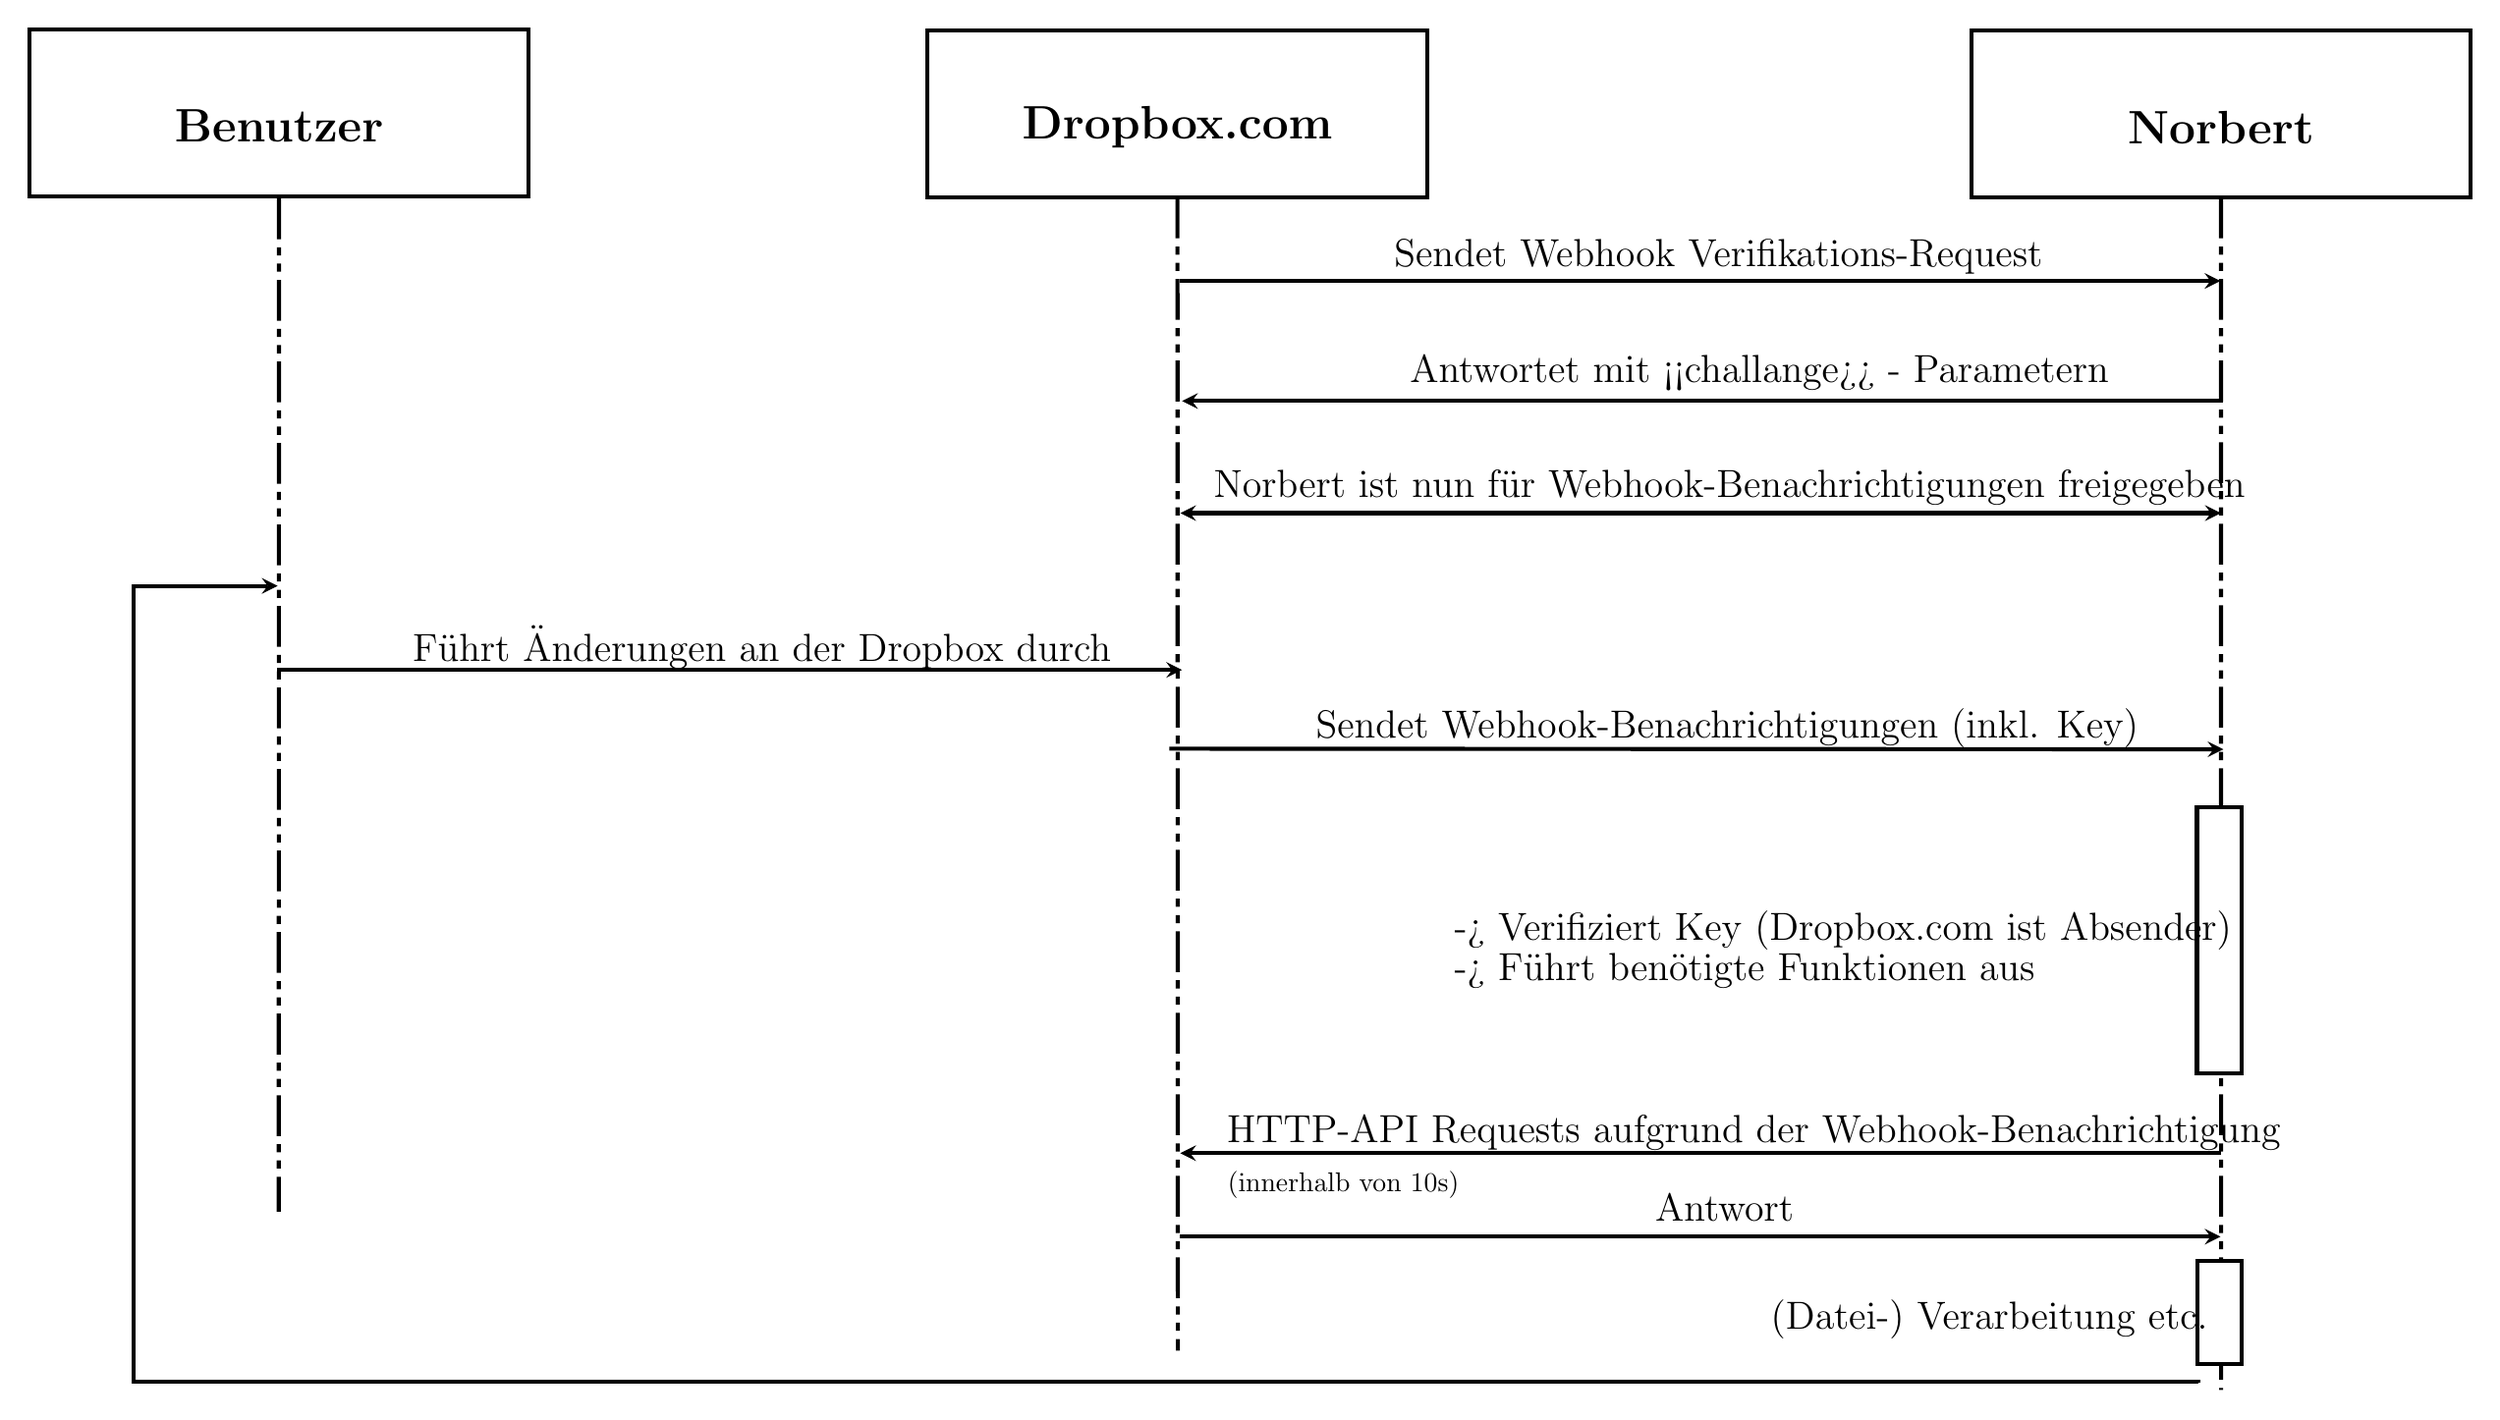
\begin{tikzpicture}
\pgftransformxscale{1.000000}
\pgftransformyscale{-1.000000}
\definecolor{dialinecolor}{rgb}{0.000000, 0.000000, 0.000000}
\pgfsetstrokecolor{dialinecolor}
\definecolor{dialinecolor}{rgb}{1.000000, 1.000000, 1.000000}
\pgfsetfillcolor{dialinecolor}
\definecolor{dialinecolor}{rgb}{1.000000, 1.000000, 1.000000}
\pgfsetfillcolor{dialinecolor}
\fill (7.350000\du,2.350000\du)--(7.350000\du,6.450000\du)--(19.600000\du,6.450000\du)--(19.600000\du,2.350000\du)--cycle;
\pgfsetlinewidth{0.100000\du}
\pgfsetdash{}{0pt}
\pgfsetdash{}{0pt}
\pgfsetmiterjoin
\definecolor{dialinecolor}{rgb}{0.000000, 0.000000, 0.000000}
\pgfsetstrokecolor{dialinecolor}
\draw (7.350000\du,2.350000\du)--(7.350000\du,6.450000\du)--(19.600000\du,6.450000\du)--(19.600000\du,2.350000\du)--cycle;
% setfont left to latex
\definecolor{dialinecolor}{rgb}{0.000000, 0.000000, 0.000000}
\pgfsetstrokecolor{dialinecolor}
\node at (13.475000\du,4.724722\du){\LARGE \textbf{Benutzer}};
\definecolor{dialinecolor}{rgb}{1.000000, 1.000000, 1.000000}
\pgfsetfillcolor{dialinecolor}
\fill (29.383000\du,2.380000\du)--(29.383000\du,6.480000\du)--(41.633000\du,6.480000\du)--(41.633000\du,2.380000\du)--cycle;
\pgfsetlinewidth{0.100000\du}
\pgfsetdash{}{0pt}
\pgfsetdash{}{0pt}
\pgfsetmiterjoin
\definecolor{dialinecolor}{rgb}{0.000000, 0.000000, 0.000000}
\pgfsetstrokecolor{dialinecolor}
\draw (29.383000\du,2.380000\du)--(29.383000\du,6.480000\du)--(41.633000\du,6.480000\du)--(41.633000\du,2.380000\du)--cycle;
% setfont left to latex
\definecolor{dialinecolor}{rgb}{0.000000, 0.000000, 0.000000}
\pgfsetstrokecolor{dialinecolor}
\node at (35.508000\du,4.754722\du){\LARGE\textbf{Dropbox.com}};
\definecolor{dialinecolor}{rgb}{1.000000, 1.000000, 1.000000}
\pgfsetfillcolor{dialinecolor}
\fill (54.975100\du,2.380000\du)--(54.975100\du,6.480000\du)--(67.225100\du,6.480000\du)--(67.225100\du,2.380000\du)--cycle;
\pgfsetlinewidth{0.100000\du}
\pgfsetdash{}{0pt}
\pgfsetdash{}{0pt}
\pgfsetmiterjoin
\definecolor{dialinecolor}{rgb}{0.000000, 0.000000, 0.000000}
\pgfsetstrokecolor{dialinecolor}
\draw (54.975100\du,2.380000\du)--(54.975100\du,6.480000\du)--(67.225100\du,6.480000\du)--(67.225100\du,2.380000\du)--cycle;
% setfont left to latex
\definecolor{dialinecolor}{rgb}{0.000000, 0.000000, 0.000000}
\pgfsetstrokecolor{dialinecolor}
\node at (61.100100\du,4.754722\du){\LARGE\textbf{Norbert}};
\pgfsetlinewidth{0.100000\du}
\pgfsetdash{{1.000000\du}{0.200000\du}{0.200000\du}{0.200000\du}{0.200000\du}{0.200000\du}}{0cm}
\pgfsetdash{{1.000000\du}{0.200000\du}{0.200000\du}{0.200000\du}{0.200000\du}{0.200000\du}}{0cm}
\pgfsetbuttcap
{
\definecolor{dialinecolor}{rgb}{0.000000, 0.000000, 0.000000}
\pgfsetfillcolor{dialinecolor}
% was here!!!
\definecolor{dialinecolor}{rgb}{0.000000, 0.000000, 0.000000}
\pgfsetstrokecolor{dialinecolor}
\draw (13.474517\du,6.499908\du)--(13.468800\du,31.357800\du);
}
\pgfsetlinewidth{0.100000\du}
\pgfsetdash{{1.000000\du}{0.200000\du}{0.200000\du}{0.200000\du}{0.200000\du}{0.200000\du}}{0cm}
\pgfsetdash{{1.000000\du}{0.200000\du}{0.200000\du}{0.200000\du}{0.200000\du}{0.200000\du}}{0cm}
\pgfsetbuttcap
{
\definecolor{dialinecolor}{rgb}{0.000000, 0.000000, 0.000000}
\pgfsetfillcolor{dialinecolor}
% was here!!!
\definecolor{dialinecolor}{rgb}{0.000000, 0.000000, 0.000000}
\pgfsetstrokecolor{dialinecolor}
\draw (35.508000\du,6.480000\du)--(35.519172\du,34.768248\du);
}
\pgfsetlinewidth{0.100000\du}
\pgfsetdash{{1.000000\du}{0.200000\du}{0.200000\du}{0.200000\du}{0.200000\du}{0.200000\du}}{0cm}
\pgfsetdash{{1.000000\du}{0.200000\du}{0.200000\du}{0.200000\du}{0.200000\du}{0.200000\du}}{0cm}
\pgfsetbuttcap
{
\definecolor{dialinecolor}{rgb}{0.000000, 0.000000, 0.000000}
\pgfsetfillcolor{dialinecolor}
% was here!!!
\definecolor{dialinecolor}{rgb}{0.000000, 0.000000, 0.000000}
\pgfsetstrokecolor{dialinecolor}
\draw (61.100100\du,6.480000\du)--(61.103237\du,35.728757\du);
}
\pgfsetlinewidth{0.100000\du}
\pgfsetdash{}{0pt}
\pgfsetdash{}{0pt}
\pgfsetbuttcap
{
\definecolor{dialinecolor}{rgb}{0.000000, 0.000000, 0.000000}
\pgfsetfillcolor{dialinecolor}
% was here!!!
\pgfsetarrowsend{stealth}
\definecolor{dialinecolor}{rgb}{0.000000, 0.000000, 0.000000}
\pgfsetstrokecolor{dialinecolor}
\draw (13.428600\du,18.067602\du)--(35.620400\du,18.067602\du);
}
% setfont left to latex
\definecolor{dialinecolor}{rgb}{0.000000, 0.000000, 0.000000}
\pgfsetstrokecolor{dialinecolor}
\node[anchor=west] at (16.482021\du,17.519877\du){\Large Führt Änderungen an der Dropbox durch};
\pgfsetlinewidth{0.100000\du}
\pgfsetdash{}{0pt}
\pgfsetdash{}{0pt}
\pgfsetbuttcap
{
\definecolor{dialinecolor}{rgb}{0.000000, 0.000000, 0.000000}
\pgfsetfillcolor{dialinecolor}
% was here!!!
\pgfsetarrowsend{stealth}
\definecolor{dialinecolor}{rgb}{0.000000, 0.000000, 0.000000}
\pgfsetstrokecolor{dialinecolor}
\draw (35.565900\du,8.525697\du)--(61.083800\du,8.525697\du);
}
% setfont left to latex
\definecolor{dialinecolor}{rgb}{0.000000, 0.000000, 0.000000}
\pgfsetstrokecolor{dialinecolor}
\node[anchor=west] at (40.555000\du,7.936172\du){\Large Sendet Webhook Verifikations-Request};
% setfont left to latex
\definecolor{dialinecolor}{rgb}{0.000000, 0.000000, 0.000000}
\pgfsetstrokecolor{dialinecolor}
\node[anchor=west] at (40.936700\du,10.771571\du){\Large Antwortet mit <<challange>> - Parametern};
\pgfsetlinewidth{0.100000\du}
\pgfsetdash{}{0pt}
\pgfsetdash{}{0pt}
\pgfsetbuttcap
{
\definecolor{dialinecolor}{rgb}{0.000000, 0.000000, 0.000000}
\pgfsetfillcolor{dialinecolor}
% was here!!!
\pgfsetarrowsstart{stealth}
\pgfsetarrowsend{stealth}
\definecolor{dialinecolor}{rgb}{0.000000, 0.000000, 0.000000}
\pgfsetstrokecolor{dialinecolor}
\draw (35.577300\du,14.220046\du)--(61.095100\du,14.220046\du);
}
% setfont left to latex
\definecolor{dialinecolor}{rgb}{0.000000, 0.000000, 0.000000}
\pgfsetstrokecolor{dialinecolor}
\node[anchor=west] at (36.126997\du,13.606820\du){\Large Norbert ist nun für Webhook-Benachrichtigungen freigegeben};
\pgfsetlinewidth{0.100000\du}
\pgfsetdash{}{0pt}
\pgfsetdash{}{0pt}
\pgfsetbuttcap
{
\definecolor{dialinecolor}{rgb}{0.000000, 0.000000, 0.000000}
\pgfsetfillcolor{dialinecolor}
% was here!!!
\pgfsetarrowsstart{stealth}
\definecolor{dialinecolor}{rgb}{0.000000, 0.000000, 0.000000}
\pgfsetstrokecolor{dialinecolor}
\draw (61.159058\du,20.014349\du)--(35.311900\du,19.999275\du);
}
% setfont left to latex
\definecolor{dialinecolor}{rgb}{0.000000, 0.000000, 0.000000}
\pgfsetstrokecolor{dialinecolor}
\node[anchor=west] at (38.635194\du,19.495575\du){\Large Sendet Webhook-Benachrichtigungen (inkl. Key)};
\pgfsetlinewidth{0.100000\du}
\pgfsetdash{}{0pt}
\pgfsetdash{}{0pt}
\pgfsetbuttcap
{
\definecolor{dialinecolor}{rgb}{0.000000, 0.000000, 0.000000}
\pgfsetfillcolor{dialinecolor}
% was here!!!
\pgfsetarrowsstart{stealth}
\definecolor{dialinecolor}{rgb}{0.000000, 0.000000, 0.000000}
\pgfsetstrokecolor{dialinecolor}
\draw (35.577275\du,29.923360\du)--(61.095075\du,29.923360\du);
}
% setfont left to latex
\definecolor{dialinecolor}{rgb}{0.000000, 0.000000, 0.000000}
\pgfsetstrokecolor{dialinecolor}
\node[anchor=west] at (36.454142\du,29.419186\du){\Large HTTP-API Requests aufgrund der Webhook-Benachrichtigung};
\pgfsetlinewidth{0.100000\du}
\pgfsetdash{}{0pt}
\pgfsetdash{}{0pt}
\pgfsetmiterjoin
\definecolor{dialinecolor}{rgb}{1.000000, 1.000000, 1.000000}
\pgfsetfillcolor{dialinecolor}
\fill (60.509117\du,21.426529\du)--(60.509117\du,27.969576\du)--(61.599625\du,27.969576\du)--(61.599625\du,21.426529\du)--cycle;
\definecolor{dialinecolor}{rgb}{0.000000, 0.000000, 0.000000}
\pgfsetstrokecolor{dialinecolor}
\draw (60.509117\du,21.426529\du)--(60.509117\du,27.969576\du)--(61.599625\du,27.969576\du)--(61.599625\du,21.426529\du)--cycle;
% setfont left to latex
\definecolor{dialinecolor}{rgb}{0.000000, 0.000000, 0.000000}
\pgfsetstrokecolor{dialinecolor}
\node[anchor=west] at (42.029945\du,24.470596\du){\Large -> Verifiziert Key (Dropbox.com ist Absender)};
% setfont left to latex
\definecolor{dialinecolor}{rgb}{0.000000, 0.000000, 0.000000}
\pgfsetstrokecolor{dialinecolor}
\node[anchor=west] at (42.029945\du,25.458374\du){\Large -> Führt benötigte Funktionen aus};
% setfont left to latex
\definecolor{dialinecolor}{rgb}{0.000000, 0.000000, 0.000000}
\pgfsetstrokecolor{dialinecolor}
\node[anchor=west] at (36.468657\du,30.691112\du){(innerhalb von 10s)};
\pgfsetlinewidth{0.100000\du}
\pgfsetdash{}{0pt}
\pgfsetdash{}{0pt}
\pgfsetmiterjoin
\definecolor{dialinecolor}{rgb}{1.000000, 1.000000, 1.000000}
\pgfsetfillcolor{dialinecolor}
\fill (60.514619\du,32.554306\du)--(60.514619\du,35.090291\du)--(61.605127\du,35.090291\du)--(61.605127\du,32.554306\du)--cycle;
\definecolor{dialinecolor}{rgb}{0.000000, 0.000000, 0.000000}
\pgfsetstrokecolor{dialinecolor}
\draw (60.514619\du,32.554306\du)--(60.514619\du,35.090291\du)--(61.605127\du,35.090291\du)--(61.605127\du,32.554306\du)--cycle;
% setfont left to latex
\definecolor{dialinecolor}{rgb}{0.000000, 0.000000, 0.000000}
\pgfsetstrokecolor{dialinecolor}
\node[anchor=west] at (59.756984\du,33.822322\du){};
% setfont left to latex
\definecolor{dialinecolor}{rgb}{0.000000, 0.000000, 0.000000}
\pgfsetstrokecolor{dialinecolor}
\node[anchor=west] at (49.785370\du,34.005671\du){\Large (Datei-) Verarbeitung etc.};
\pgfsetlinewidth{0.100000\du}
\pgfsetdash{}{0pt}
\pgfsetdash{}{0pt}
\pgfsetmiterjoin
\pgfsetbuttcap
{
\definecolor{dialinecolor}{rgb}{0.000000, 0.000000, 0.000000}
\pgfsetfillcolor{dialinecolor}
% was here!!!
\pgfsetarrowsend{stealth}
{\pgfsetcornersarced{\pgfpoint{0.000000\du}{0.000000\du}}\definecolor{dialinecolor}{rgb}{0.000000, 0.000000, 0.000000}
\pgfsetstrokecolor{dialinecolor}
\draw (60.553240\du,35.528758\du)--(60.553240\du,35.520959\du)--(59.614751\du,35.520959\du)--(59.614751\du,35.520959\du)--(35.714589\du,35.520959\du)--(35.714589\du,35.520959\du)--(9.905243\du,35.520959\du)--(9.905243\du,16.004850\du)--(13.440770\du,16.004850\du);
}}
\pgfsetlinewidth{0.100000\du}
\pgfsetdash{}{0pt}
\pgfsetdash{}{0pt}
\pgfsetbuttcap
{
\definecolor{dialinecolor}{rgb}{0.000000, 0.000000, 0.000000}
\pgfsetfillcolor{dialinecolor}
% was here!!!
\pgfsetarrowsstart{stealth}
\definecolor{dialinecolor}{rgb}{0.000000, 0.000000, 0.000000}
\pgfsetstrokecolor{dialinecolor}
\draw (35.622205\du,11.470399\du)--(61.140105\du,11.470399\du);
}
\pgfsetlinewidth{0.100000\du}
\pgfsetdash{}{0pt}
\pgfsetdash{}{0pt}
\pgfsetbuttcap
{
\definecolor{dialinecolor}{rgb}{0.000000, 0.000000, 0.000000}
\pgfsetfillcolor{dialinecolor}
% was here!!!
\pgfsetarrowsend{stealth}
\definecolor{dialinecolor}{rgb}{0.000000, 0.000000, 0.000000}
\pgfsetstrokecolor{dialinecolor}
\draw (35.569172\du,31.969303\du)--(61.087072\du,31.969303\du);
}
% setfont left to latex
\definecolor{dialinecolor}{rgb}{0.000000, 0.000000, 0.000000}
\pgfsetstrokecolor{dialinecolor}
\node[anchor=west] at (46.956556\du,31.25\du){\Large Antwort};
\end{tikzpicture}
}
%	\caption{API-Zugriffe über die Dropbox-Endpoints}
%	\label{04ergebnis:webhook}	
%\end{figure}